%!TEX root = ../TTK4550-MHT.tex
\section{Results}
\label{sec:results}

\subsection{Testing scheme}
The evaluation of the MHT algorithm is two-sided, firstly the algorithm must be able to track under challenging conditions, secondly it must be able to do this without having an ever growing computationally cost. The first performance metric is how well the algorithm is estimating the true position to the object it is tracking. This is measured as the two-dimensional distance:
\begin{equation}
	\Delta P = \| \V{p}_{track}-\V{p}_{target} \|_2
\end{equation}
where the track is considered correct if $\Delta P \leq	\varepsilon_p$ for all t after initial convergence. If a track is deviating more that the threshold and is never within the threshold again, it is considered lost at the time-step it exceeded the threshold. If the track should converge after exceeding the threshold, it is considered restored at the time-step it is returning within the limit. The algorithm is tested on five scenarios:
\begin{itemize}
	\item Five fully cooperating ships
    \item Five partially cooperatic ships
    \item Five ships avoiding obsticles with large space
    \item Five ships avoiding obsticles with little space
	\item Five parallel ships
\end{itemize}

\begin{figure}
    \centering
    \begin{minipage}{0.49\textwidth}
        \centering
        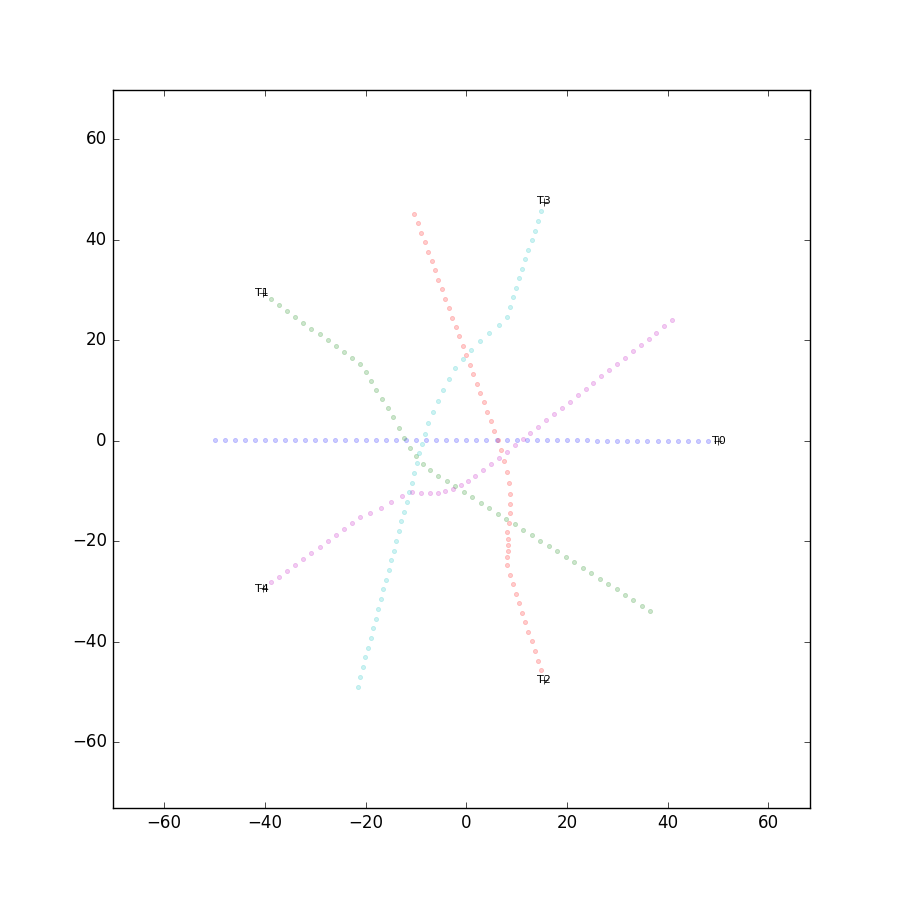
\includegraphics[clip, trim=2cm 1.5cm 2cm 2cm, width=\textwidth]{scenario1}
        \caption{First scenario}
    \end{minipage}
    \begin{minipage}{0.49\textwidth}
        \centering
        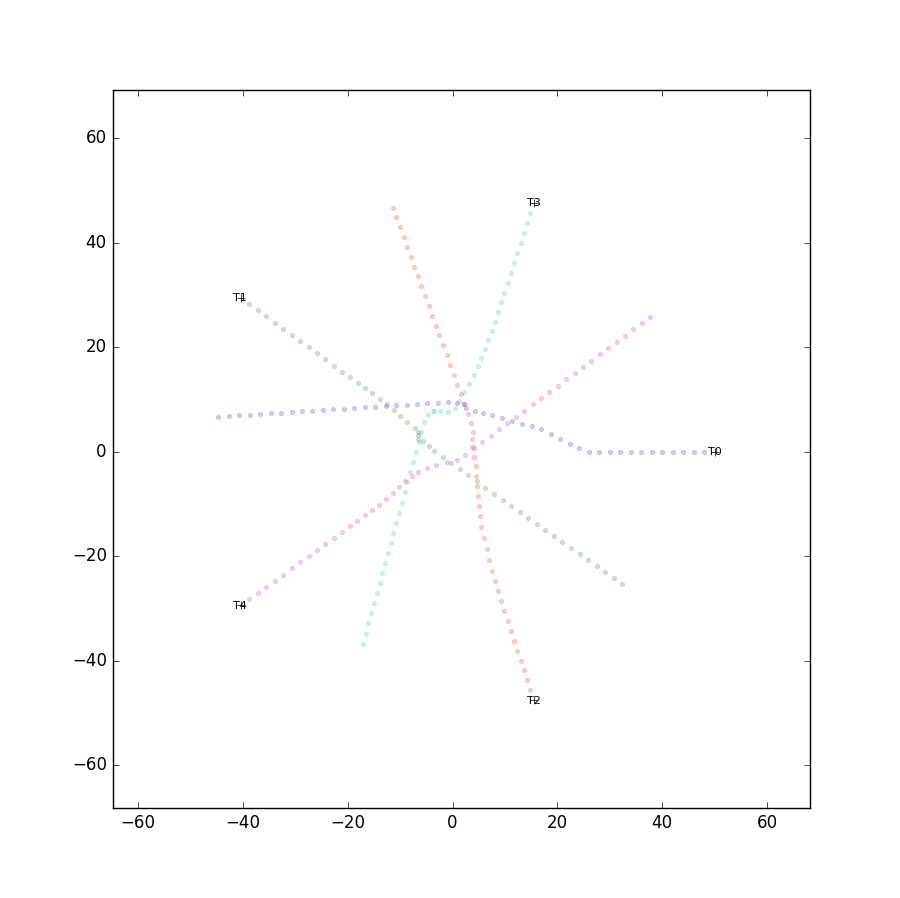
\includegraphics[clip, trim=2cm 1.5cm 2cm 2cm,width=\textwidth]{scenario2}
        \caption{Second scenario}
    \end{minipage}
\end{figure}
\begin{figure}
    \centering
    \begin{minipage}{0.49\textwidth}
        \centering
        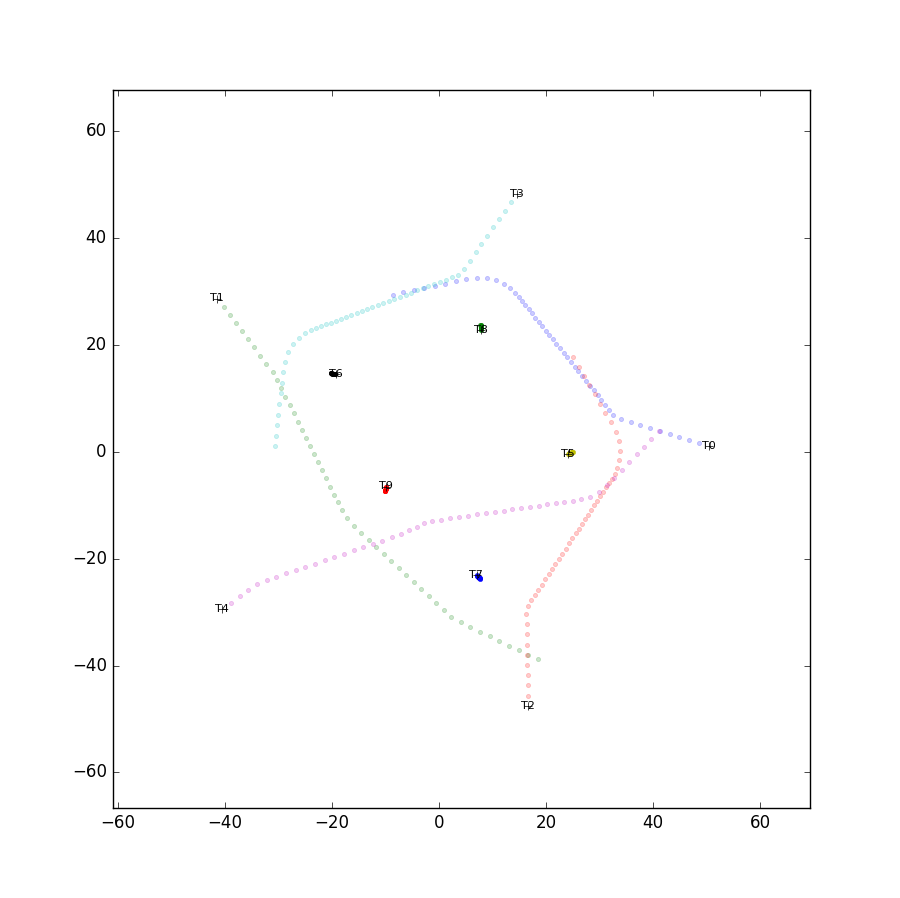
\includegraphics[clip, trim=2cm 1.5cm 2cm 2cm,width=\textwidth]{scenario3}
        \caption{Third scenario}
    \end{minipage}
    \begin{minipage}{0.49\textwidth}
        \centering
        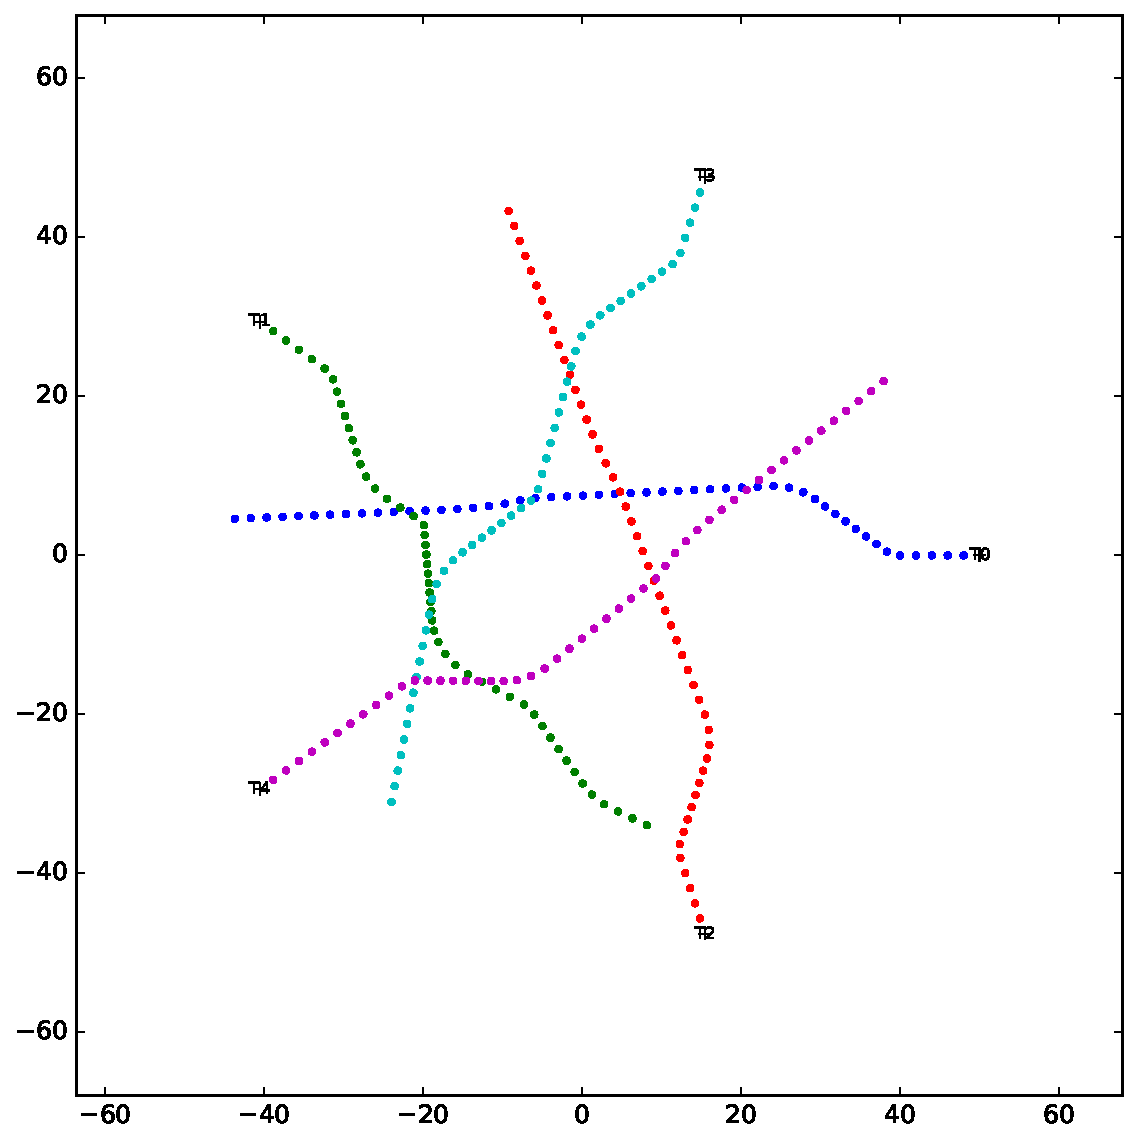
\includegraphics[clip, trim=2cm 1.5cm 2cm 2cm,width=\textwidth]{scenario4}
        \caption{Fourth scenario}
    \end{minipage}
\end{figure}
\begin{figure}
    \centering
    \begin{minipage}{0.49\textwidth}
        \centering
        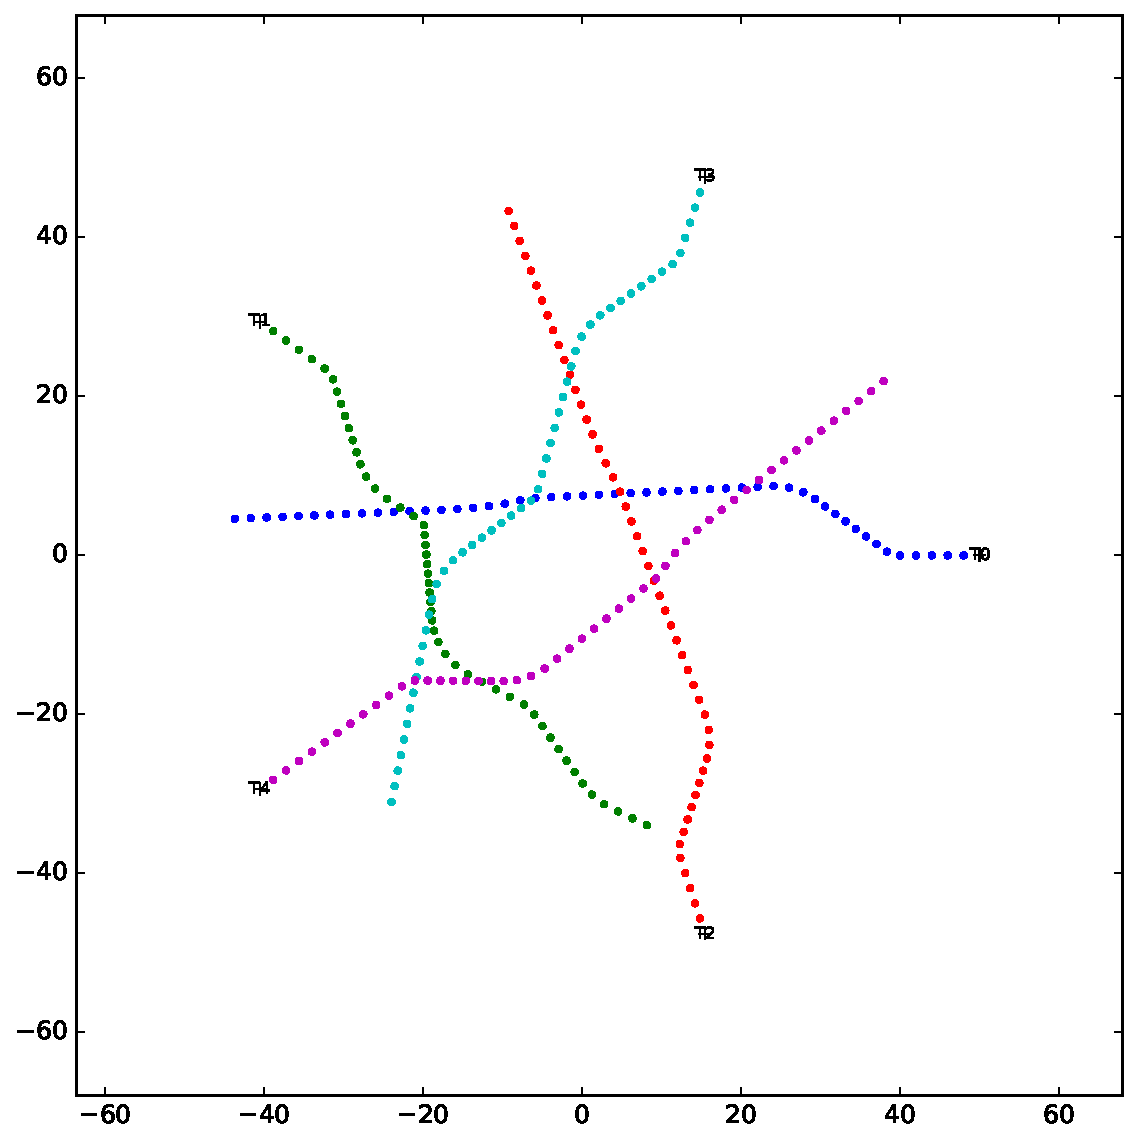
\includegraphics[clip, trim=2cm 1.5cm 2cm 2cm,width=\textwidth]{scenario4}
        \caption{Fifth scenario}
    \end{minipage}
\end{figure}

\subsection{Simulation data}
The first data-set is time and position extracted from an Autonomous Surface Vessel (ASV)-simulator with collision avoidance (COLAV) [Giorgio]. The targets are configured such that they need to maneuver to avoid collision with each other. This allows for tracking of maneuvering targets in close proximity to each other. The second data-set is linear parallel paths with hight measurements noise and system uncertainty. The third data-set is generated from Thomas Stenersen ASV simulator which was a part of this masters thesis. This simulator have several different pre-configured scenarios, and can also be modified to create any desired scenario.

\subsection{Tracking performance}
Scenario 1 was simulated with the following variations

\begin{tabular}{ r c c c c c c}
N 	& $\lambda_\phi$ & GLPK 	& CBC	& SYMPHONY	& Gurobi	& Xpress	\\ \hline
1 	& 0.111	& 6 	& 6		& 6			& 6			& 6			\\
3 	& 0.106	& 9		& 9		& 6			& 6			& 6			\\
5 	& 0.106	& 9		& 9		& 6			& 6			& 6			\\
7 	& 0.108	& 9		& 9		& 6			& 6			& 6			\\
\end{tabular}

\subsection{Runtime}
\subsubsection{Solvers}

\begin{tabular}{ r c c c c c c}
nHyp 	& CPLEX & GLPK 	& CBC	& SYMPHONY	& Gurobi	& Xpress	\\ \hline
13 		& 0.111	& 6 	& 6		& 6			& 6			& 6			\\
34 		& 0.106	& 9		& 9		& 6			& 6			& 6			\\
78 		& 0.106	& 9		& 9		& 6			& 6			& 6			\\
87 		& 0.108	& 9		& 9		& 6			& 6			& 6			\\
162 	& 0.112	& 9		& 9		& 6			& 6			& 6			\\
189 	& 0.115	& 9		& 9		& 6			& 6			& 6			\\
423 	& 0.130	& 9		& 9		& 6			& 6			& 6			\\
\end{tabular}